\documentclass[convert,border=1cm]{standalone}
\usepackage[x11names, rgb]{xcolor}
\usepackage[utf8]{inputenc}
\usepackage{tikz}
\usetikzlibrary{snakes,arrows,shapes}
\usepackage{amsmath}
%
%
%
%
\begin{document}
% White background.
\pagecolor[RGB]{255,255,254}
%
%

% Start of code
% \begin{tikzpicture}[anchor=mid,>=latex,join=bevel,]
\begin{tikzpicture}[>=latex,join=bevel,]
\pgfsetlinewidth{1bp}
\Large%
21
\begin{scope}
  \definecolor{strokecol}{rgb}{0.0,0.0,0.0};
  \pgfsetstrokecolor{strokecol}
  \draw (91bp,11.5bp) node {Linear Model};
\end{scope}
\begin{scope}
  \pgfsetstrokecolor{black}
  \definecolor{strokecol}{rgb}{1.0,1.0,1.0};
  \pgfsetstrokecolor{strokecol}
  \definecolor{fillcol}{rgb}{1.0,1.0,1.0};
  \pgfsetfillcolor{fillcol}
  \filldraw (0bp,0bp) -- (0bp,102bp) -- (182bp,102bp) -- (182bp,0bp) -- cycle;
  \definecolor{strokecol}{rgb}{0.0,0.0,0.0};
  \pgfsetstrokecolor{strokecol}
  \draw (91bp,11.5bp) node {Linear Model};
\end{scope}
\begin{scope}
  \pgfsetstrokecolor{black}
  \definecolor{strokecol}{rgb}{1.0,1.0,1.0};
  \pgfsetstrokecolor{strokecol}
  \definecolor{fillcol}{rgb}{1.0,1.0,1.0};
  \pgfsetfillcolor{fillcol}
  \filldraw (0bp,0bp) -- (0bp,102bp) -- (182bp,102bp) -- (182bp,0bp) -- cycle;
  \definecolor{strokecol}{rgb}{0.0,0.0,0.0};
  \pgfsetstrokecolor{strokecol}
  \draw (91bp,11.5bp) node {Linear Model};
\end{scope}
  \pgfsetcolor{black}
  % Edge: x1 -> output
  \definecolor{newcol}{hsb}{0,0,0.9};
  \pgfsetcolor{newcol}
  \draw [->] (36.084bp,43.491bp) .. controls (60.767bp,47.091bp) and (106.65bp,53.782bp)  .. (145.94bp,59.512bp);
  \definecolor{strokecol}{rgb}{0.9,0.9,0.9};
  \pgfsetstrokecolor{strokecol}
  \draw (91bp,60.5bp) node[text=black!10] {0.3949};
  % Edge: x0 -> output
  \definecolor{newcol}{hsb}{0,0,0};
  \pgfsetcolor{newcol}
  \draw [->] (36.084bp,81.39bp) .. controls (60.767bp,77.619bp) and (106.65bp,70.609bp)  .. (145.94bp,64.607bp);
  \definecolor{strokecol}{rgb}{0.0,0.0,0.0};
  \pgfsetstrokecolor{strokecol}
  \draw (91bp,82.5bp) node[text=black!100] {75.75};
  % Node: output
\begin{scope}
  \definecolor{strokecol}{rgb}{1.0,0.0,0.0};
  \pgfsetstrokecolor{strokecol}
  \draw [solid] (164bp,62bp) ellipse (18bp and 18bp);
  \definecolor{strokecol}{rgb}{0.0,0.0,0.0};
  \pgfsetstrokecolor{strokecol}
  \draw (164bp,62bp) node {$h(\mathbf{x})$};
\end{scope}
  % Node: x0
\begin{scope}
  \definecolor{strokecol}{rgb}{0.0,0.0,0.0};
  \pgfsetstrokecolor{strokecol}
  \draw [solid] (18bp,84bp) ellipse (18bp and 18bp);
  \draw (18bp,84bp) node[font=\huge] {$x_0$};
\end{scope}
  % Node: x1
\begin{scope}
  \definecolor{strokecol}{rgb}{0.0,1.0,0.0};
  \pgfsetstrokecolor{strokecol}
  \draw [solid] (18bp,41bp) ellipse (18bp and 18bp);
  \definecolor{strokecol}{rgb}{0.0,0.0,0.0};
  \pgfsetstrokecolor{strokecol}
  \draw (18bp,41bp) node[font=\huge] {$x_{1}$};
\end{scope}
%
\end{tikzpicture}
% End of code

%
\end{document}
%
<<startfigonlysection>>
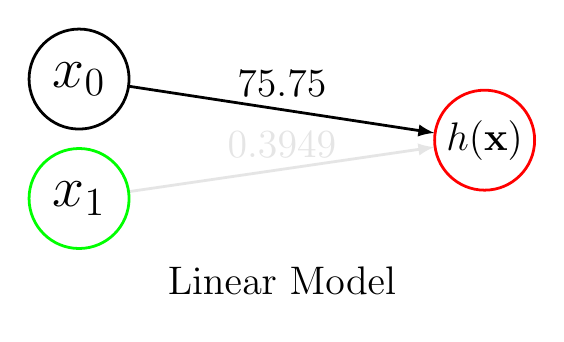
\begin{tikzpicture}[>=latex,join=bevel,]
\pgfsetlinewidth{1bp}
\Large%
\begin{scope}
  \definecolor{strokecol}{rgb}{0.0,0.0,0.0};
  \pgfsetstrokecolor{strokecol}
  \draw (91bp,11.5bp) node {Linear Model};
\end{scope}
\begin{scope}
  \pgfsetstrokecolor{black}
  \definecolor{strokecol}{rgb}{1.0,1.0,1.0};
  \pgfsetstrokecolor{strokecol}
  \definecolor{fillcol}{rgb}{1.0,1.0,1.0};
  \pgfsetfillcolor{fillcol}
  \filldraw (0bp,0bp) -- (0bp,102bp) -- (182bp,102bp) -- (182bp,0bp) -- cycle;
  \definecolor{strokecol}{rgb}{0.0,0.0,0.0};
  \pgfsetstrokecolor{strokecol}
  \draw (91bp,11.5bp) node {Linear Model};
\end{scope}
\begin{scope}
  \pgfsetstrokecolor{black}
  \definecolor{strokecol}{rgb}{1.0,1.0,1.0};
  \pgfsetstrokecolor{strokecol}
  \definecolor{fillcol}{rgb}{1.0,1.0,1.0};
  \pgfsetfillcolor{fillcol}
  \filldraw (0bp,0bp) -- (0bp,102bp) -- (182bp,102bp) -- (182bp,0bp) -- cycle;
  \definecolor{strokecol}{rgb}{0.0,0.0,0.0};
  \pgfsetstrokecolor{strokecol}
  \draw (91bp,11.5bp) node {Linear Model};
\end{scope}
  \pgfsetcolor{black}
  % Edge: x1 -> output
  \definecolor{newcol}{hsb}{0,0,0.9};
  \pgfsetcolor{newcol}
  \draw [->] (36.084bp,43.491bp) .. controls (60.767bp,47.091bp) and (106.65bp,53.782bp)  .. (145.94bp,59.512bp);
  \definecolor{strokecol}{rgb}{0.9,0.9,0.9};
  \pgfsetstrokecolor{strokecol}
  \draw (91bp,60.5bp) node[text=black!10] {0.3949};
  % Edge: x0 -> output
  \definecolor{newcol}{hsb}{0,0,0};
  \pgfsetcolor{newcol}
  \draw [->] (36.084bp,81.39bp) .. controls (60.767bp,77.619bp) and (106.65bp,70.609bp)  .. (145.94bp,64.607bp);
  \definecolor{strokecol}{rgb}{0.0,0.0,0.0};
  \pgfsetstrokecolor{strokecol}
  \draw (91bp,82.5bp) node[text=black!100] {75.75};
  % Node: output
\begin{scope}
  \definecolor{strokecol}{rgb}{1.0,0.0,0.0};
  \pgfsetstrokecolor{strokecol}
  \draw [solid] (164bp,62bp) ellipse (18bp and 18bp);
  \definecolor{strokecol}{rgb}{0.0,0.0,0.0};
  \pgfsetstrokecolor{strokecol}
  \draw (164bp,62bp) node {$h(\mathbf{x})$};
\end{scope}
  % Node: x0
\begin{scope}
  \definecolor{strokecol}{rgb}{0.0,0.0,0.0};
  \pgfsetstrokecolor{strokecol}
  \draw [solid] (18bp,84bp) ellipse (18bp and 18bp);
  \draw (18bp,84bp) node[font=\huge] {$x_0$};
\end{scope}
  % Node: x1
\begin{scope}
  \definecolor{strokecol}{rgb}{0.0,1.0,0.0};
  \pgfsetstrokecolor{strokecol}
  \draw [solid] (18bp,41bp) ellipse (18bp and 18bp);
  \definecolor{strokecol}{rgb}{0.0,0.0,0.0};
  \pgfsetstrokecolor{strokecol}
  \draw (18bp,41bp) node[font=\huge] {$x_{1}$};
\end{scope}
%
\end{tikzpicture}
<<endfigonlysection>>
